\section*{Introduzione}
Prima di entrare nel dettaglio della nostra trattazione definiamo che cos'è un \emph{Linguaggio Formale.} Innanzitutto dobbiamo distinguere tra un \emph{linguaggio natura} ed uno \emph{artificiale}, un linguaggio naturale è quello che utiliziamo tutti i giorni e che si basa sul significato delle parole e soprattutto non possiede una struttura formale. Un linguaggio artificiale, invece, è quello utilizzato per la comunicazione tra macchine, è di tipo no verbale ma soprattutto è formale.\\
Un linguaggio si definisce \textbf{formale} se la sua \emph{sintassi} (ovvero la sua struttura) e la sua \emph{semantica} (ovvero il suo significato) sono definiti da precisi algoritmi. Questo permette di definire delle \emph{procedure} precise per determinare la correttezza di una frase che appartiene ad un linguaggio e il suo significato. 
In un contesto più ristretto un \textbf{linguaggio formale} è un \emph{oggetto matematico} costruito su di un \emph{alfabeto} tramite regole assiomatiche chiamate \emph{grammatiche} o tramite strumenti matematici chiamati \emph{automi}.\\
\section{Introduzione alla teoria dei linguaggi formali}
Vediamo ora alcune definizioni che ci saranno utili durante il corso:
\begin{description}
	\item[Alfabeto:] insieme \emph{finito} di elementi
	$$\Sigma = \{a_1, a_2, a_3, \dots, a_k\}$$
	\item[Cardinalità di un alfabeto:]  è il numero di elementi che lo compongono
	$$ |\Sigma| = k $$
	\item[Stringa:] insieme ordinato di elementi dell'alfabeto che possono essere anche ripetuti.
	$$\Sigma = \{a,b,c\}$$
	$$Stringe: \ abc \vee aab \vee ac \vee bbb$$
	\item[Linguaggio:] insieme finito o infinito di stringhe di un alfabeto
	$$L_1 = \{ab,ac,abc\}$$
	$$L_2 = \{bc,bbc,\dots\}$$
	La struttura insiemistica del linguaggio formale ha due livelli di profondità:
	\begin{itemize}
		\item Insieme non ordinato di elementi non atomici (\emph{stringhe}) che sono
		\item sequenze ordinate di elementi atomici (\emph{elementi o terminali}).
	\end{itemize}
	\item[Cardinalità di un linguaggio:] può essere finita o infinita.
	$$|L_1| = |\{ab,ac,abc\}| = 3$$
	\item[Lunghezza di una stringa:] indica il numero dei suoi elementi
	$$|abb| = 3 \quad |abbc| = 4$$
	\item[Uguaglianza tra stringhe:] due stringhe si definiscono uguali se e solo se hanno la stessa lunghezza, ed i suoi elementi coincidono ordinatamente da sinistra a destra.
	$$x = a_1a_2\dots a_h \quad y = b_1b_2\dots b_k$$
	$$x = y \iff h = k \wedge a_i = b_i \ \forall i = 1\to h $$
\end{description}
\subsection{Operazioni sulle stringhe}
La \emph{concatenazione} è l'operazione fondamentale con le stringhe, si tratta di fare il prodotto tra esse. Questa operazione è un operazione di base e non fa altro che disporre in fila le due stringhe.
$$x = a_1a_2\dots a_h \quad y = b_1b_2\dots b_k$$
$$x\cdot y = a_1a_2\dots a_hb_1b_2\dots b_k = xy$$
Questo tipo di operazione gode della proprietà associativa e va ad influire sulla lunghezza della stringa come vediamo dalla \ref{eq:conass} e dalla \ref{eq:conlen}.
\begin{equation}\label{eq:conass}
	(xy)z = x(yz)
\end{equation}
\begin{equation}\label{eq:conlen}
	|xyz| = |x| + |y| + |z|
\end{equation}
La concatenazione ci permette di introdurre un altro concetto relativo alle stringhe, ovvero quello della \emph{stringa vuota} o \emph{nulla} indicata con $ \varepsilon $ questa stringa è l'elemento neutro rispetto all'operazione di concatenazione, infatti, concatenando $ \varepsilon $ a destra o a sinistra di una stringa la stringa non cambia.
$$\varepsilon x = x\varepsilon = x$$
Tuttavia bisogna prestare attenzione a non confondere la stringa nulla con l'insieme vuoto $\varnothing$.\\
Una volta capita l'operazione di concatenazione si possono individuare in una stringa delle \emph{sotto-stringhe}, ovvero stringhe più piccole concatenate tra loro per formare una stringa più grande.
Ad esempio data una stringa $x$ essa può essere vista come un insieme di sotto-stringhe concatenate
$$x = uyv$$
Dove:
\begin{itemize}
	\item \emph{y} è detta sotto-stringa.
	\item \emph{u} è chiamato prefisso.
	\item \emph{v} è chiamato suffisso.
\end{itemize}
Un esempio di suffissi, prefissi e sotto-stringhe è mostrato in \figurename\,\ref{fig:sufpref}.
\begin{figure}
	\centering
	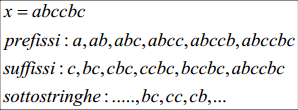
\includegraphics[width=0.5\linewidth]{img/substr.png}
	\caption{Esempio di sottostringhe con prefissi e suffissi}\label{fig:sufpref}
\end{figure}

Si definiscono \emph{sotto-stringhe proprie} tutte quelle stringhe che hanno $u\neq \varepsilon$ e $v \neq \varepsilon$.\\
La \emph{riflessione} è l'operazione che inverte l'ordine dei caratteri che compongono una stringa. Da quanto si vede in \figurename \ref{fig:riflessione} notiamo che la riflessione gode di alcune proprietà, la riflessione di una stringa riflessa ci riporta alla stringa originale, la riflessione di due stringhe concatenate è uguale alla riflessione delle singole stringhe e successivamente la loro concatenazione, infine la riflessione della stringa vuota è uguale ancora alla stringa vuota.
\begin{figure}
	\centering
	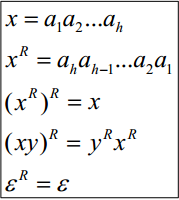
\includegraphics[width=0.3\linewidth]{img/riflessione.png}
	\caption{Proprietà della riflessione}\label{fig:riflessione}
\end{figure}
La \emph{ripetizione} o anche \emph{iterazione} è quell'operazione che permette di concatenare più volte una stringa con se stessa; dato un indice $ m $ maggiore di uno allora la ripetizione non fa altro che concatenare \emph{m}-volte la stringa con se stessa come si vede dalla \figurename \ref{fig:ripetizione}.
\begin{figure}
	\centering
	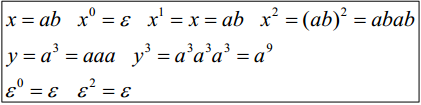
\includegraphics[width=0.65\linewidth]{img/ripetizione.png}
	\caption{Esempio di ripetizione}\label{fig:ripetizione}
\end{figure}
Come nel caso dell'algebra classica anche qui abbiamo una precedenza tra le operazioni, in particolare la \emph{ripetizione} ha precedenza sulla \emph{concatenazione}, anche la \emph{riflessione} ha precedenza sulla \emph{concatenazione}.\\
\subsection{Operazioni sui linguaggi}
Prima di tutto dobbiamo definire che cosa vuol dire effettuare un'operazione su di un linguaggio. In realtà effettuare un'operazione si di un linguaggio significa effettuare tale operazione su tutte le stringhe appartenenti a quel linguaggio.
Ad esempio effettuare la riflessione di un linguaggio significa:
$$L^R = \{x|x= y^R\wedge y \in L\}$$
Ovvero si viene a creare un nuovo linguaggio di stringhe \emph{x} che non sono altro che la riflessione di tutte le stringhe \emph{y} del linguaggio di partenza.\\
Un altro esempio è il linguaggio definito come \emph{prefisso(L)} ovvero:
$$prefisso(L) = \{y|x = yz \wedge x\in L \wedge y,z \neq \varepsilon\}$$
Da questa definizione possiamo definire un linguaggio \emph{prefix-free} nel quale non esiste una stringa appartenente a questo linguaggio che sia prefisso di un'altra stringa dello stesso linguaggio.
$$L_1 = \{x | x = a^nb^n \wedge n\geq 1\}$$
Ad esempio:
$$a^2b^2 \in L_1 \quad a^2b \notin L_1$$
Passiamo ora a definire le \emph{operazioni binarie} ovvero quelle composte da due operandi come la \emph{concatenazione} tra due linguaggi.
$$L'\cdot L''= \{xy | x\in L' \wedge y \in L''\}$$
Da questa definizione possiamo anche dimostrare la ripetizione di un linguaggio tramite la \ref{eq:lenpot}
\begin{equation}\label{eq:lenpot}
\left\{
	\begin{array}{lcc}
	L^m = L^{m-1}\cdot L & se & m>0\\
	L^m = \{\varepsilon\} & se & m = 0
	\end{array}
	\right.
\end{equation}
Una cosa molto importante da ricordare è la differenza tra la stringa nulla $ \varepsilon $ e il linguaggio vuoto $ \varnothing $, infatti abbiamo che:
$$L\cdot \varnothing = \varnothing \cdot L = \varnothing$$
mentre
$$L \cdot \{\varepsilon\} = \{\varepsilon\}\cdot L = L $$
Dalla definizione di potenza di un linguaggio possiamo ricavare la possibilità di definire un secondo linguaggio che contiene tutte le stringhe che hanno lunghezza minore di un determinato numero \emph{k} che è la potenza del linguaggio. Ad esempio:
$$L = \{\varepsilon,a,b\}^3 \quad k = 3$$
$$L = \{\varepsilon,a,b,aa,ab,bb,aaa,\dots , bbb\}$$
L'utilizzo della stringa nulla $ \varepsilon $ ci permette di esprimere le stringhe di lunghezza \emph{1} e \emph{2}.\\
Oltre alle normali operazioni definiamo anche le operazioni insiemistiche sui linguaggi. Tali operazioni sono l'\emph{unione} ($ \cup $), l'\emph{intersezione} ($ \cap $), la \emph{differenza} ($ \setminus $), l'\emph{inclusione} ($ \subseteq $), l'\emph{inclusione stretta} ($ \subset $) e l'\emph{uguaglianza} ($ = $).\\
Dopo aver introdotto queste operazioni possiamo definire il \emph{linguaggio universale} come insieme di tutte le stringhe di alfabeto $ \Sigma $
$$L_{universale} = \Sigma^0 \cup \Sigma^1 \cup \Sigma^2 \cup \dots$$
$$L_{universale} = \neg \varnothing$$
Il \emph{complemento} di un linguaggio \emph{L} di alfabeto $ \Sigma $ è definito come la differenza insiemistica tra il \emph{linguaggio universale} e il linguaggio \emph{L} ovvero:
$$\neg L = L_{universale}\setminus L$$
ed indica l'insieme delle stringhe di alfabeto $ \Sigma $ e che non appartengono a \emph{L}.\\
Sia nel linguaggio naturale che in quello artificiale le stringhe possono avere una qualsiasi lunghezza, tuttavia per definire un linguaggio è necessario utilizzare formule di lunghezza finita. Risulta perciò necessario introdurre alcuni operatori per creare delle stringhe infinite.
L'operatore \emph{star} noto anche come \emph{stella di Kleene} indica la chiusura \emph{riflessiva} e \emph{transitiva} rispetto al concatenamento. Questo operatore indica l'unione di tutte le potenze del linguaggio e si indica come:
$$L^\ast=\bigcup_{h=0\dots\infty}L^h = L^0\cup L^1 \cup L^2 \dots = \varepsilon \cup L^1 \cup L^2 \dots $$
Un esempio di un linguaggio finito è $L = \{ab,ba\}$ che diventa infinito una volta applicato l'operatore stella:
$$L^\ast = \{\varepsilon,ab,ba,abba,abab,baba,baab,\dots\}$$
Tuttavia è anche possibile che il linguaggio iniziale \emph{L} ed il linguaggio $ L^\ast $ coincidano.
$$L= \{a^{2n}| n\geq 0\} \quad L^\ast = \{a^{2n}| n\geq 0\} \equiv L$$
Ogni stringa del linguaggio $ L^\ast $ può essere suddivisa in una sotto-stringa del linguaggio $ L $.\\
Se prendiamo un alfabeto $ \Sigma $ come base di un linguaggio, $ \Sigma^\ast $ contiene tutte le stringhe ($ \Sigma^\ast $ è il linguaggio universale). Si può anche dire che L è un linguaggio costruito sull'alfabeto $ \Sigma $ tramite la notazione $ L\subseteq \Sigma^\ast$.
L'operatore \emph{stella} possiede alcune proprietà importanti:
\begin{itemize}
	\item monotonicità
	$$L\subseteq L^\ast$$
	\item chiusura rispetto al concatenamento
	$$se \ \ (x\in L^\ast \wedge y \in L^\ast) \Rightarrow xy \in L^\ast$$
	\item idempotenza
	$$(L^\ast)^\ast = L^\ast$$
	\item commutatività di stella e riflessione
	$$(L^R)^\ast = (L^\ast)^R$$
\end{itemize}
Inoltre applicando l'operazione stella al linguaggio vuoto e alla stringa nulla otteniamo che:
$$\varnothing^\ast = \{\varepsilon\} \qquad \{\varepsilon\}^\ast = \{\varepsilon\}$$
Un esempio di idempotenza è già stato mostrato ed era:
$$L= \{a^{2n}| n\geq 0\} \quad L^\ast = \{a^{2n}| n\geq 0\} \equiv L$$
questo perché il linguaggio \emph{L} può essere visto come:
$$L=L_0* \ dove \ L_0 = \{aa\}$$
L'operatore \emph{croce} è la \emph{chiusura transitiva} rispetto al concatenamento, ovvero è l'unione delle potenze tranne la potenza \emph{0}; in molti casi è molto utile tuttavia non è indispensabile in quanto deriva dall'operatore stella.
$$L^+ = \bigcup_{h=1\dots\infty}=L^1\cup L^2\cup L^3 \dots$$
Operatore \emph{quoziente} ($ / $) accorcia una frase di un primo linguaggio eliminando un suffisso appartenete ad un secondo linguaggio. \begin{center}
	\textit{Notare che a differenza dell'operatore differenza la barra in questo caso è rivolta in avanti}
\end{center}
$$L=L'/L''=\{y|(x=yz \in L') \wedge z \in L''\}$$
Un esempio di questo utilizzo è:
$$L' = \{a^{2n}b^{2n}|n>0\}, \quad L'' = \{b^{2n+1} | n \geq 0 \}$$
$$
\begin{array}{rcl}
L'/L'' & = & \{a^rb^s | (r\geq , pari) \wedge (1\leq s <r, s \ dispari)\}\\
& = & \{a^2b, a^4b,a^4b^3, \dots\}
\end{array}
$$
